\subsection{Introduction}
Serval\footnote{More information about the Serval Architecture can be found in the presentation in the Appendix (\ref{sec:servaldhtpres}).} is an end-host stack and a service-centric network architecture, proposed and prototyped by the \href{https://sns.cs.princeton.edu/}{systems and networking group} at \href{https://www.princeton.edu}{Princeton University}, in 2012.

\paragraph{} In the original paper "A Service Access Layer, at Your Service" (2011)\cite{Freedman2011} and later on "Serval: An End-Host Stack for Service-Centric Networking" (2012)\cite{Nordstrom2012}, Nordstr{\"o}m et. al. first decompose the needs of modern networked applications, locate the discordances with the current Network Stack, study previous work and how each of them individually fails to stand as a proper solution, reconsider the current TCP/IP Networking Stack and propose two simple abstractions that can obliterate the legacy problems discussed on Problem Definition\ref{problemdefinition}.\\
\indent Furthermore they introduce 	

\subsection{Proposed abstractions}



\subsection{Serval Network Stack}
\subsubsection{Service Controller}
\subsubsection{Service Access Layer}
\subsection{Service Resolution in the Serval architecture}

\subsection{Application portability and incremental deployment}
- A translator can be used but: (ADD SCHEMA)
works as an intermediate
slows down performance
apps still work with the traditional apis
 -- adds complexity, translator will have to support many versions/protocols and error proof for them
 -- reimplements the functionality already working on SAL


\subsection{Incremental migration to Serval}
With Serval being actively under development, it is time to discuss the deployment approaches that could guide us to something that has never happened before; the wide adoption of a new network stack.
Above all, benchmarks prove that introducing Serval in large scale networks as well as datacenters offers a wide range of new functionality in speeds comparable to the original TCP/IP stack ones. However, with Internet being a massive diverse network controlled distributively by assorted interest groups --vendors, ISPs, service providers--, deployment of a new networking architecture is a real nightmare \cite{Podmayersky2011}.
\\ \indent Prime example is the adoption of IPv6. Intending to solve the problem of IPv4 exhaustion, IPv6 uses 128-bit addresses (in comparison to IPv4's 32-bit IP addresses), providing approximately 4.3 billion addresses for network interfaces. Still, after over a decade of protracted efforts, less than 4\% \footnote{Visualization based on original data from RIR, routeviews, Alexa, Google, ITU and APnic by Cisco at \url{http://6lab.cisco.com/stats/}} of Internet global traffic is carried over it, although it is a necessary to take step for the next generation of the Internet of Things. \nomenclature{IoT}{Internet of Things}
\\ \indent A smooth transition to a new architecture requires two things: first that current hardware and intermediary devices are compatible or at least do not interfere with the new packet headers, and that applications are utilizing the late interfaces and are able to dissect and synthesize those packets.

\subsubsection{Legacy Hardware}
SAL's position just on top of the network layer makes it translucent to networking equipment such as hubs, switches and routers, since they are messing up with the headers of up to the network layer.
At this level, hardware is responsible only for delivering the packets to the right destination, the way they have been doing so far.
\\ \indent Serval on the contrary is not immune to stateful packet inspection\nomenclature{SPI}{Stateful Packet Inspection} and deep packet inspection\nomenclature{DPI}{Deep Packet Inspection}.
Intermediaries who access the headers of the transport or above layers will have a hard time dissecting a minimum 32 extra bytes following the network layer.
The use of NAT-based\nomenclature{NAT}{Network Address Translator} agents though, such as load balancers, can be obscured due to the late binding on serviceIDs.
In any way, operation behind legacy networks middleware can be achieved via UDP encapsulation.
\\ \indent Apparently, even if typical routers are compatible with routing Serval packets, they cannot provide service-level routing, service registration, unregistration and propagation, or any other feature of a Serval router\footnote{The generation of routers that supports virtual services, such as the Cisco Nexus series 1100, might be able to imitate features of a service router with a virtual service.}.
Hopefully this is not a blocking obstacle, as far as the SAL knows a service router that can forward service name resolution requests to.
That service router might be deep within the network and not accessible through service propagation.

\subsubsection{Modified Programming Interfaces}
Unlike other proposals which can be either integrated in programs as libraries or provide abstractions by overloading identifiers such as ports, Serval's kernel module implementation requires applications to be modified in order to use its active sockets API.
\\ \indent In other words, a minimum port of an existing applications would require to include and link to \textless libserval/serval.h\textgreater ~and \textless netinet/serval.h\textgreater ~libraries, set socket family to AF\_SERVAL and substitute system calls to the socket layer such as connect, bind, accept, send etc to use serviceIDs.
Minor modifications might be needed, since new identifiers require different size of bytes to be allocated in memory and so on.
\\ \indent The complexity of porting an existing application to Serval depends on how neatly is the connection module isolated.
In general, applications that support various protocols are easier to be ported, since connectivity functions are already decoupled from the program logic and can be replicated to support new APIs.
Large applications, with thousands lines of code,\nomenclature{loc}{lines of code} like Mozilla Firefox require modifications in around just 70 lines of code.
Design patterns like singleton and factory noticeably indicate which parts of the source code should be altered.
\\ \indent Nevertheless, applications can simultaneously support multiple protocols and stacks, according to the requests of the other end.
This will be a great advantage in the transitory period of large scale deployment.
\\ \indent On the other hand, unexpected runtime results might be confronted due to overlapping of features offered by SAL and reimplemented in the program.
For instance service load balancing at SAL, an inherent component of Serval, might muddle with the application-specific way of allotting requests.
In such cases if possible one of the methods should dominate the final decision.
Either a unique serviceID of an allocated serviceID block --as described in the Hierarchical Resolution approach-- should be used for each instance, and let load-balancing be made by application's functions.
Or load-balancing logic within the application should be removed when a socket's family is AF\_SERVAL and be managed according to service-level rules defined in SAL.
\\ \indent As a reference you can find a diff file from the port of nginx\footnote{Nginx [engine-ex] is an Open Source HTTP, reverse proxy and mail proxy server\\ \url{http://nginx.org/}.} to Serval in the appendix \ref{sec:nginxport}.
This diff version includes the integration of the [nginx\_1.2.9\_serval\_fqdn] branch commits from \mbox{sns/Serval} repository into the build procedure.

\subsubsection{Incremental Deployment with Serval translator}
\begin{figure}
\centering
\captionsetup{justification=centering}
\phantomsection
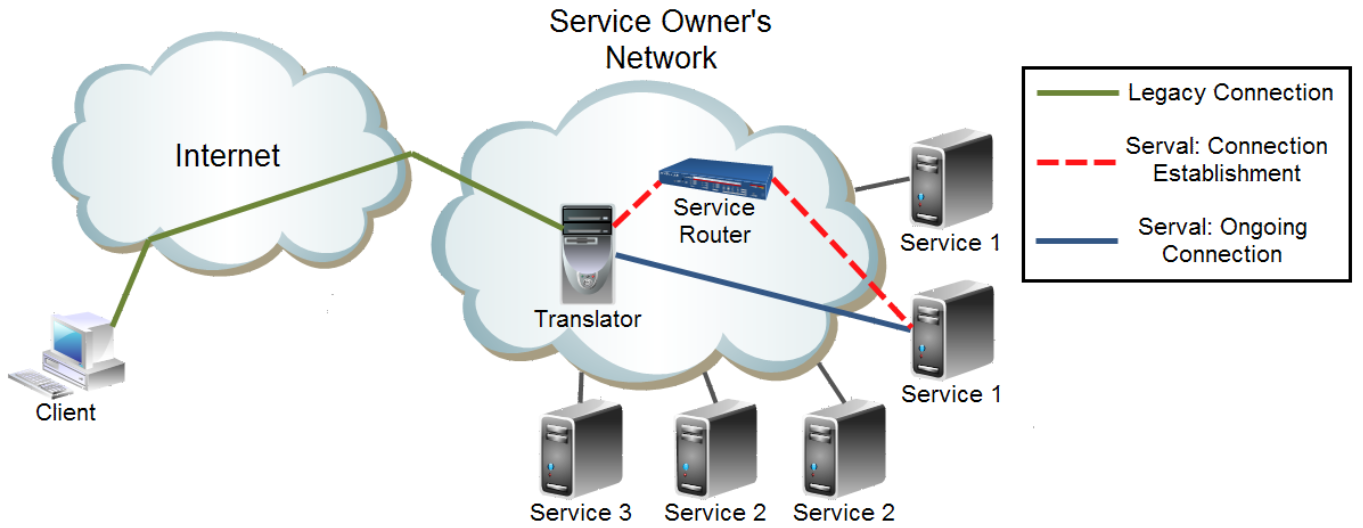
\includegraphics[scale=0.25]{figures/Serval_translator}
\caption[Serval translator]{A Serval translator as an intermediary\\for communicating with legacy clients \cite{Podmayersky2011}.}
\label{fig:serval_translator}
\end{figure}
The Internet has expanded in a level where migrating to a new architecture through a coordinated "flag day", where we disconnect all devices in order to cold-plug update them, is an unnegoatiable scenario.
Downtime, unreachable hosts running on embedded hardware, telecommunications, are only a few of the reasons that induce a gradual strategy when it comes to adopting Serval.
\\ \indent As observed in similar examples, the ones expected to make the first move are service providers.
Both for the reason that they are greatly benefited by this migration, as well for their pertinent awareness.
In order to face the challenge of serving both legacy and Serval-enabled clients, Brandon Podmayersky implements a \emph{Serval translator} \cite{Podmayersky2011}, an intermediary service which can be hosted in a middlebox machine or on the server itself, and which bridges the connection between a service using Serval active sockets and legacy TCP/IP clients.
\\ \indent Serval translator works on the simple principle of exposing legacy TCP/IP interfaces to the outer network --may it be the Internet--, which are then translated to Serval active sockets.
The procedure is illustrated in Figure~\ref{fig:serval_translator}.
Legacy clients resolving a service name via a search mechanism, may it be DNS, get the public-facing IP address of the translator in front of the corresponding service.
Then they are connecting with that IP and a well-known port directly to the Serval translator, opening a typical AF\_INET socket.
The predefined port as anyone would expect can be the default legacy port of the service the client wants to reach (for a web server that would be port 80).
Note that a translator might be the first point of contact for multiple services, with its IP address registered --similar to a DNS A record-- for various service names and mapping requests to different ports to different services or service instances.
This mapping actually links an $<IP, port>$ tuple to a serviceID, which then can be resolved using the service table of SAL, or custom load balancing rules. 
After that, the translator takes care of the connection synchronization with the service, and splices\footnote{splice() is a system call introduced in the 2.6.17 kernel, that can move data between two file descriptors without copying between kernel address space and user address space\\ \url{http://linux.die.net/man/2/splice}.}
When the connection is terminated, the translator closes the sockets at both ends.
\\ \indent Using the Serval translator a service provider can handle requests from both legacy and Serval-ready clients.
Requests that have a serviceID get routed directly to the service instance, overpassing the translator.
However, on an established legacy connection, every single packet is processed by the translator, modifying headers and flags appropriately.
This indeed adds an overhead and indicates a possible single point of failure, but benchmarks show its performance is good enough to be deployed in real networks and a cluster of such translators can be used in a hierarchical schema.

\subsection{Profiling the Serval prototype implementation}
Among the admirable headliners of Serval is the working prototype version of the proposed architecture.
In more than 28000 lines of code\footnote{Source code is open source and can be found in their public repository\\ \url{https://github.com/princeton-sns/serval/}.} covering functionality of the Service Access Layer (both in userlevel operation and as a Linux kernel module), bindings for multiple programming languages, a translator, libraries and examples for writing serval compatible applications, and with a reported throughput comparable to the unmodified TCP/IP stack, it is clearly showcased the feasibility of the solution.\\
\indent In this section we are profiling the prototype in regard to the following parameters:
\begin{enumerate}
  \item Memory Management
  \item CPU Instructions and Cycles
  \item System Calls times
  \item Execution time needed for the completion of a numbered iteration of requests
  \item The sum of requests that can be satisfied within a given timeframe
\end{enumerate}
Then we will be graphically presenting the results juxtaposed to the measurements of the unchanged TCP/IP stack and the AF\_INET family. The first four tests have not been published before.
\paragraph{} Output was obtained on a ...... machine running Ubuntu 11.04 (Natty Narwahl) kernel version 2.6.38-16-generic (rebuilt with debug symbols). Serval was built with --enable-debug option for the first three tests.\\
For the measurements we ported the nginx\footnote{Nginx [engine-ex] is an Open Source HTTP,reverse proxy and mail proxy server\\ \url{http://nginx.org/}.} web server to serval architecture, integrating the [nginx\_1.2.9\_serval\_fqdn] branch commits into the build procedure. Also, we implemented a simple HTTP client which supports both AF\_INET and the AF\_SERVAL socket families, depending on the options passed during the call. Source code of both can be found in the Appendix (\ref{sec:sourcecode}).


\iffalse
gprof
perf
google-profile tools
1) memory (oprofile)
2) CPU cycles (callgrind)
3) system calls time (strace)
4) timed execution of 1000 times
5) requests per second
6) Number of packers per request, bytes sent, packet structure
\fi

TODO: Complete this section, maybe add HIP, Chord and OpenFlow